% Propósito: hacer visible la secuencia cuadrado-promedio-raíz que define el
% RMS y diferenciarla del valor medio de la presión.
% Origen: p/p_hat=sin(2 pi t/T),
% overline{p}=0, overline{p^2}/p_hat^2=1/2 y
% p_rms/p_hat=1/sqrt(2), ecuaciones \eqref{eq:u4-presion-media},
% \eqref{eq:u4-presion-rms} y \eqref{eq:u4-rms-sinusoide}.
% Curvas teóricas normalizadas; no representan datos medidos.
% Descripción accesible: el panel superior muestra una sinusoide con media
% cero y picos positivos y negativos. El panel inferior muestra su cuadrado,
% siempre no negativo, cuya media normalizada es un medio. Al tomar la raíz
% de esa media se obtiene un RMS igual al pico dividido por raíz de dos.
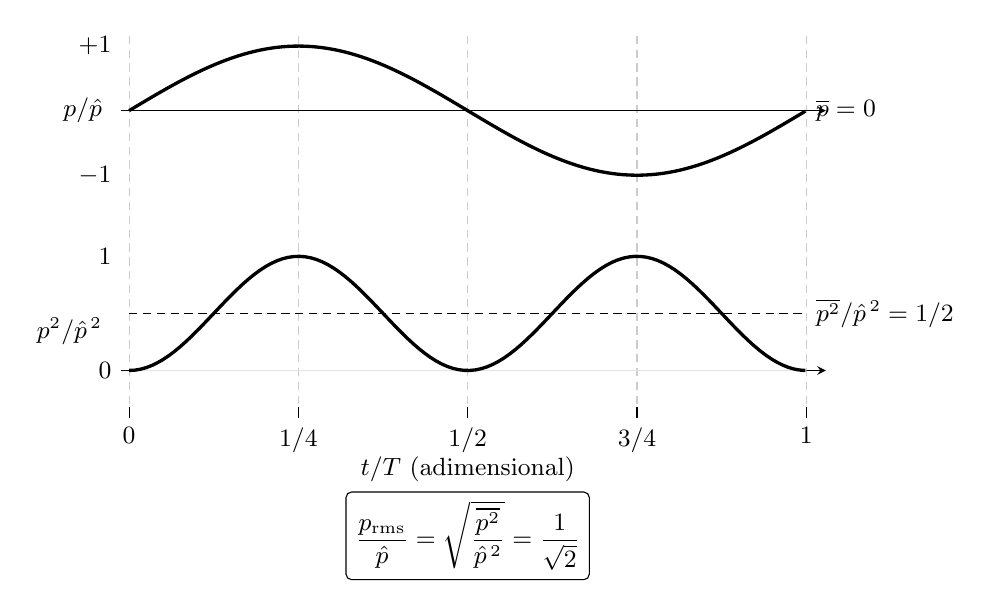
\begin{tikzpicture}[font=\small,>=stealth,x=1cm,y=1cm]
    \foreach \q/\lab in {0/{0},0.25/{1/4},0.5/{1/2},0.75/{3/4},1/{1}}{
        \pgfmathsetmacro{\xx}{2.10+8.6*\q}
        \draw[densely dashed,black!20] (\xx,-1.05) -- (\xx,3.85);
        \draw (\xx,-1.05) -- (\xx,-0.92);
        \node[below] at (\xx,-1.05) {\(\lab\)};
    }

    \draw[->] (2.00,2.85) -- (10.95,2.85);
    \draw[->] (2.00,-0.45) -- (10.95,-0.45);
    \node[anchor=east] at (1.88,2.85) {\(p/\hat p\)};
    \node[anchor=east,align=right] at (1.88,0.05)
        {\(p^2/\hat p^{\,2}\)};

    \draw[very thick,samples=120,domain=0:1]
        plot ({2.10+8.6*\x},{2.85+0.82*sin(360*\x)});
    \draw[densely dashed] (2.10,2.85) -- (10.70,2.85)
        node[anchor=west] {\(\overline p=0\)};
    \node[anchor=east] at (2.00,3.67) {\(+1\)};
    \node[anchor=east] at (2.00,2.03) {\(-1\)};

    \draw[black!10] (2.10,-0.45)
        plot[samples=120,domain=0:1]
        ({2.10+8.6*\x},{-0.45+1.45*(sin(360*\x))^2})
        -- (10.70,-0.45) -- cycle;
    \draw[very thick,samples=120,domain=0:1]
        plot ({2.10+8.6*\x},{-0.45+1.45*(sin(360*\x))^2});
    \draw[densely dashed] (2.10,0.275) -- (10.70,0.275)
        node[anchor=west] {\(\overline{p^2}/\hat p^{\,2}=1/2\)};
    \node[anchor=east] at (2.00,1.00) {\(1\)};
    \node[anchor=east] at (2.00,-0.45) {\(0\)};

    \node at (6.40,-1.70) {\(t/T\) (adimensional)};
    \node[draw,rounded corners=2pt,fill=white] at (6.40,-2.55)
        {\(\displaystyle
          \frac{p_\mathrm{rms}}{\hat p}
          =\sqrt{\frac{\overline{p^2}}{\hat p^{\,2}}}
          =\frac{1}{\sqrt{2}}\)};
\end{tikzpicture}
